\section{Cycle}

%%%%%%%%%%%%%%%
\begin{frame}{Cycle detection}
  \begin{table}[ht]
    \centering
    \caption{Cycle detection \pno{3.4.21}}
    \begin{tabular}{c||c|c}
     \hline
     		& Digraph 			& Undirected graph  \\ \hline \hline
		DFS 	& back edge \textcolor{red}{$\iff$} cycle 	
			& back edge $\iff$ cycle 
			\\ \hline
		BFS	& \begin{tabular}[c]{@{}l@{}}back edge $\Rightarrow$ cycle\\ cycle \textcolor{red}{$\nRightarrow$} back edge \end{tabular} 
			& cross edge $\iff$ cycle  
			\\ \hline
    \end{tabular}
  \end{table}
\end{frame}
%%%%%%%%%%%%%%%
\begin{frame}{Cycle detection}
  \begin{block}{Solution.}
    \begin{columns}[t]
      \column{0.50\textwidth}
	DFS on digraph: $\text{cycle} \Rightarrow \text{back edge}$
	\begin{figure}
	  \centering
	  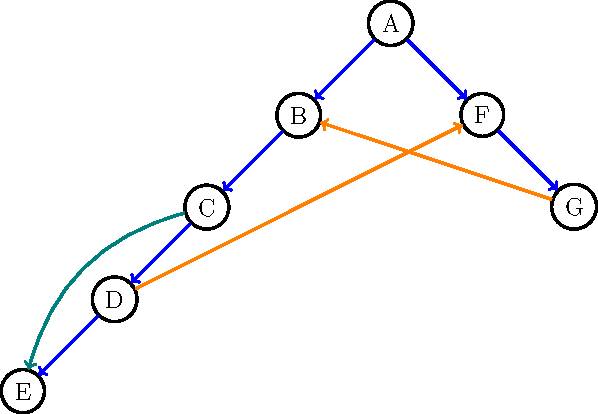
\includegraphics[width=0.50\textwidth]{figures/dfs-digraph-cycle-detection-without-back.pdf}
	\end{figure}
      \column{0.50\textwidth}
	BFS on digraph: $\text{cycle} \nRightarrow \text{back edge}$
	\begin{figure}
	  \centering
	  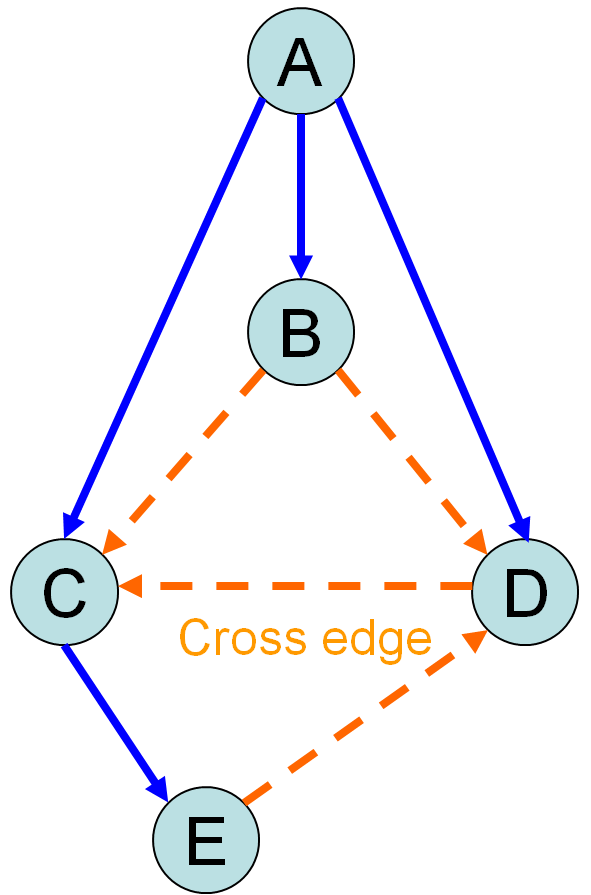
\includegraphics[width=0.30\textwidth]{figures/bfs-digraph-cycle-without-back.png}
	\end{figure}
      \end{columns}
  \end{block}

  \begin{alertblock}{Remark.}
    \begin{itemize}
      \item cycle in undirected graphs (shortly)
      \item cycle in digraphs $\Rightarrow$ DAG, SCC
    \end{itemize}
  \end{alertblock}
\end{frame}
%%%%%%%%%%%%%%%
\begin{frame}{Edge deletion}
  \begin{exampleblock}{Edge deletion \pno{3.4.12}}
    \begin{itemize}
      \item Input: connected, undirected graph $G$
      \item Problem: $\exists? e \in E: G \setminus e$ is connected?
      \item $O(|V|)$
    \end{itemize}
  \end{exampleblock}

  \begin{block}{Solution.}
    cycle $\iff \exists e$:
    \begin{proof}
      \begin{itemize}
	\item $\Leftarrow$: by contradiction. connected + acyclic $\Rightarrow$ tree
      \end{itemize}
    \end{proof}

    tree: $|E| = |V| - 1$ $\Rightarrow$ check $|E| \ge |V|$
  \end{block}
\end{frame}
%%%%%%%%%%%%%%%
\begin{frame}{Orientation of undirected graph}
  \begin{exampleblock}{Orientation of undirected graph \pno{3.4.13}}
    Undirected (connected) graph $G$, edge oriented s.t. $\forall v, \text{in}[v] \ge 1$.
  \end{exampleblock}

  \begin{block}{Solution.}
    orientation $\iff$ $\exists$ cycle; DFS
  \end{block}
\end{frame}
%%%%%%%%%%%%%%%
\begin{frame}{Bipartite graph}
  \begin{exampleblock}{Bipartite graph \pno{3.4.26; 3.4.32}}
    To test bipartiteness of an undirected graph.
  \end{exampleblock}

  \begin{block}{Solution.}
    \begin{columns}
      \column{0.40\textwidth}
        BFS + Coloring:
	\begin{itemize}
	  \item pick any $s$, c[s] = 0
	  \item $u \gets \text{Dequeue}(Q)$
	  \item $\forall (u,v)$: 
	    \begin{itemize}
	      \item tree edge
	      \item cross edge: \textcolor{red}{check}
	    \end{itemize}
	\end{itemize}
      \column{0.60\textwidth}
	\begin{proof}
	  Check cross edge $(u,v)$:
	  \begin{itemize}
	    \item ($\exists$) $d[v] = d[u]$ $\Rightarrow$ the same layer $\Rightarrow$ odd cycle (\pno{3.4.17}; \textcolor{red}{EX}) $\Rightarrow$ non-bipartite
	    \item ($\forall$) $d[v] = d[u] + 1$ $\Rightarrow$ different layers $\Rightarrow$ different colors
	  \end{itemize}
	\end{proof}
    \end{columns}
  \end{block}
\end{frame}
%%%%%%%%%%%%%%%
